\begin{textblock*}{\posterboxwidth / 5}(0cm,0cm)

\def\figscale{.6}
\def\figfontsize{\small}

\newcommand\tikzbox[1]{%
\scalebox{\figscale}{%
\begin{tikzpicture}[font=\figfontsize]
\input{#1}
\end{tikzpicture}}%
}

\centering%
\textbf{Comparison of approximations: coverage C}\\[.5em]

\tikzbox{vector/QualityMeasures_C1}\\
\tikzbox{vector/QualityMeasures_C2}

\end{textblock*}


\begin{textblock*}{\posterboxwidth / 5}(\posterboxwidth * 4 / 5,0cm)

\def\figscale{.6}
\def\figfontsize{\small}

\newcommand\tikzbox[1]{%
\scalebox{\figscale}{%
\begin{tikzpicture}[font=\figfontsize]
\input{#1}
\end{tikzpicture}}%
}

\centering%
\textbf{Comparison of approximations: R measure}\\[.5em]

\tikzbox{vector/QualityMeasures_R1}\\
\tikzbox{vector/QualityMeasures_R2}

\end{textblock*}


\begin{textblock*}{\posterboxwidth * 3 / 5}(\posterboxwidth / 5,-0.7cm)%
\centering%
\begin{tabular}{lll}
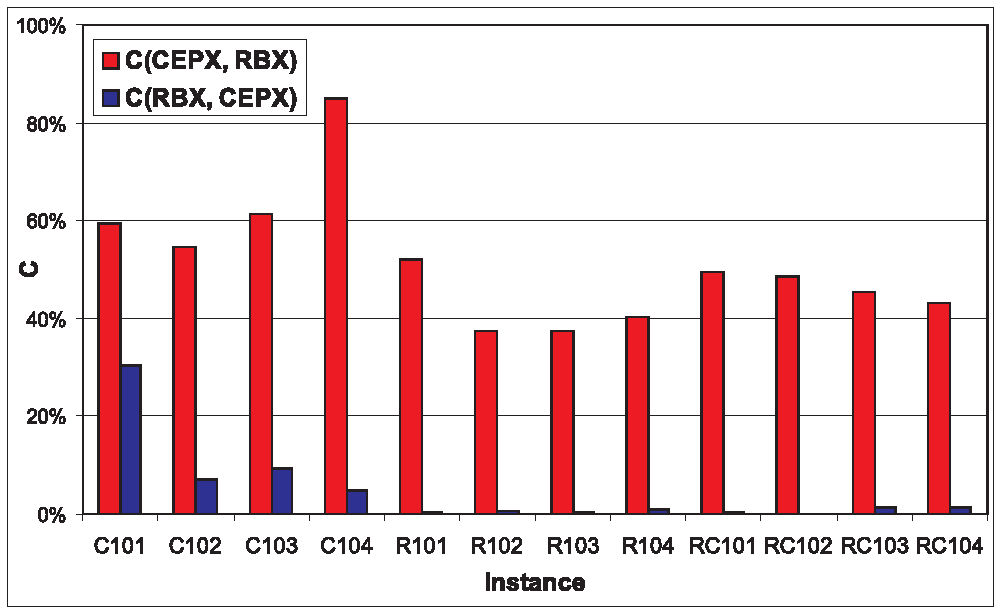
\includegraphics[height=\posterboxheight * 6/10]{vector/Comparison_C}&\hspace{2em}&%
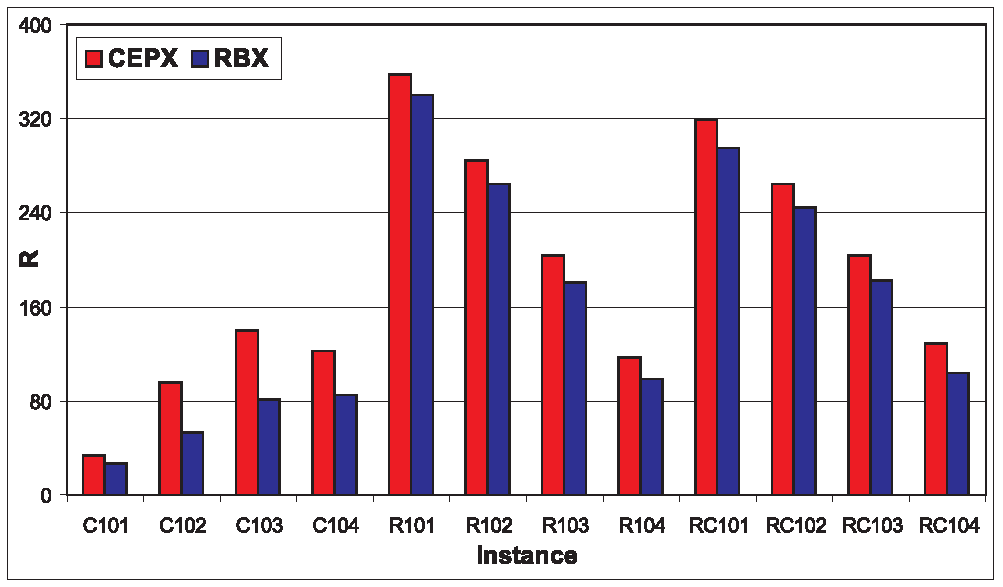
\includegraphics[height=\posterboxheight * 6/10]{vector/Comparison_R}\\
\hspace{1em}\parbox[t]{\posterboxwidth / 4}{%
	Comparison of instances:
	\begin{mylist}
	\item clustered instances are easier than random ones
	\item wide time window $\rightarrow$ easier random instances
	\item wide time window $\rightarrow$ harder clustered instances
	\end{mylist}%
}& &% 
\hspace{1em}\parbox[t]{\posterboxwidth / 4}{%
	Comparison of crossovers:
	\begin{mylist}
	\item RBX is random, CEPX is deterministic
	\item RBX is usually better than CEPX
	\item randomness in RBX is useful
	\end{mylist}%
}
\end{tabular}
\end{textblock*}
